
\documentclass{article}
\usepackage[utf8]{inputenc}
\usepackage{hyperref}
\usepackage[margin=0.75in]{geometry}
\usepackage{tikz}
\usetikzlibrary{shapes.geometric,arrows}
\tikzstyle{startstop} = [rectangle, rounded corners, minimum width = 3cm, minimum height = 1cm,text centered, draw = black ,fill = red!30]
\tikzstyle{io} = [trapezium, trapezium left angle = 70, trapezium right angle =110, minimum width = 3cm, minimum height = 1cm, text centered, draw=black, fill=blue!30]
\tikzstyle{process} = [rectangle, minimum width = 3cm, minimum height = 1cm, text centered,draw = black, fill= orange!30]
\tikzstyle{decision} = [diamond, minimum width =3cm, minimum height = 1cm text centered, draw = black, fill=green!30]
\tikzstyle{arrow} = [thick,->,>=stealth]
\begin{document}
	\begin{center}
    
    	% MAKE SURE YOU TAKE OUT THE SQUARE BRACKETS
    
		\LARGE{\textbf{Idea Proposal}} \\
        \vspace{1em}
        \Large{Simple Approach to Improving Industry Work-Flow Efficiency} \\
        \vspace{1em}
        \normalsize\textbf{Shafkat Waheed} \\
        \normalsize\textbf{Adnan chowdhury} \\
        \vspace{1em}
        \normalsize{Advisor: 
Mohammad Ashrafuzzaman Khan
} \\
        \vspace{1em}
        \normalsize{North South University} \\
        \normalsize{Bachelors of Science in Computer Science and Engineering}
     
	\end{center}
    \begin{normalsize}
    
    	\section{Objective:}
        
        The main objective of this idea is to develop a system that would enable the our garments industry to increase their production efficiency with minimal invasion. 
  
      
		\section{Challenges:}
        
       The garments factory produce most of their commodity through a strict regiment of steps that should be maintained constantly to deliver its products within a certain deadline.But this continuous flow of production is hampered due to \textbf{ human error}, \textbf{ loss of durability of machines}.The side effects of this problems are poor quality product,temporary shutdown of production and sudden disruption of production flow.   
        
	   	\section{Causes:}
        
      Firstly, human error is caused by inexperienced workers, irresponsible workers, work-load, personal issues, satisfactions due to low payment.Among this reasons \textbf{work-load} and \textbf{inexperience worker} influence human error.
      
      loss of durability of machines are mainly caused due to improper maintenance of machines. Machines are continuously running to produce commodity at an steady rate, as the production flow continuous efficiency of machines deteriorate day by day giving rise to faulty components in mechanical and electrical parts of the machines.
      
       \section{Approach:}
        
      Firstly, human error can be reduced in production flow by building an A.I that would constantly monitor the parameters defined by the human workers in production through a camera. The A.I would monitor the parameters and also would predict what would be the final output of production based on parameters defined by the workers.This would take pressure off workers who are given heavy work load and safe guard against irresponsible workers in case of their clumsy mistake. 
      
      Secondly,loss of durability of machines are well know by experienced workers, and this experience in handling machines enables them to schedule maintenance task for machines used for production, this experience also helps them to stay prepared in case any disastrous failure of machines.Like the workers its also possible to detect faults and problems in machines using A.I and Predict disastrous machines failure.Some article regarding how to detect this faults.
        
        \begin{itemize}
        
\item(1)\href{https://www.rsipvision.com/machine-fault-detection-and-classification/}{RISP Vision On Fault Detection} 
\item(2)\href{https://medium.com/bigdatarepublic/machine-learning-for-predictive-maintenance-where-to-start-5f3b7586acfb}{Medium Article on Fault Detection} 
\item(3)\href{https://arxiv.org/pdf/1901.08247.pdf}{Machine Learning and Deep Learning
Algorithms for Bearing Fault Diagnostics}

        \end{itemize}
        
    	\section{Possible Issues:}
        Possible problems to face are collection of data in the case of detecting faults in machines and how dynamic is the process production.
        \section{Work Flow of different Industry  :}
        Different types of industry produces different products but the work flow of all the industry follows a simple pattern. All this industries use machines which are operated by human personnel, this machines are prone to human error if not properly monitored. examples of some work environments and its human interaction.
        \subsection{abul khayer steel}
        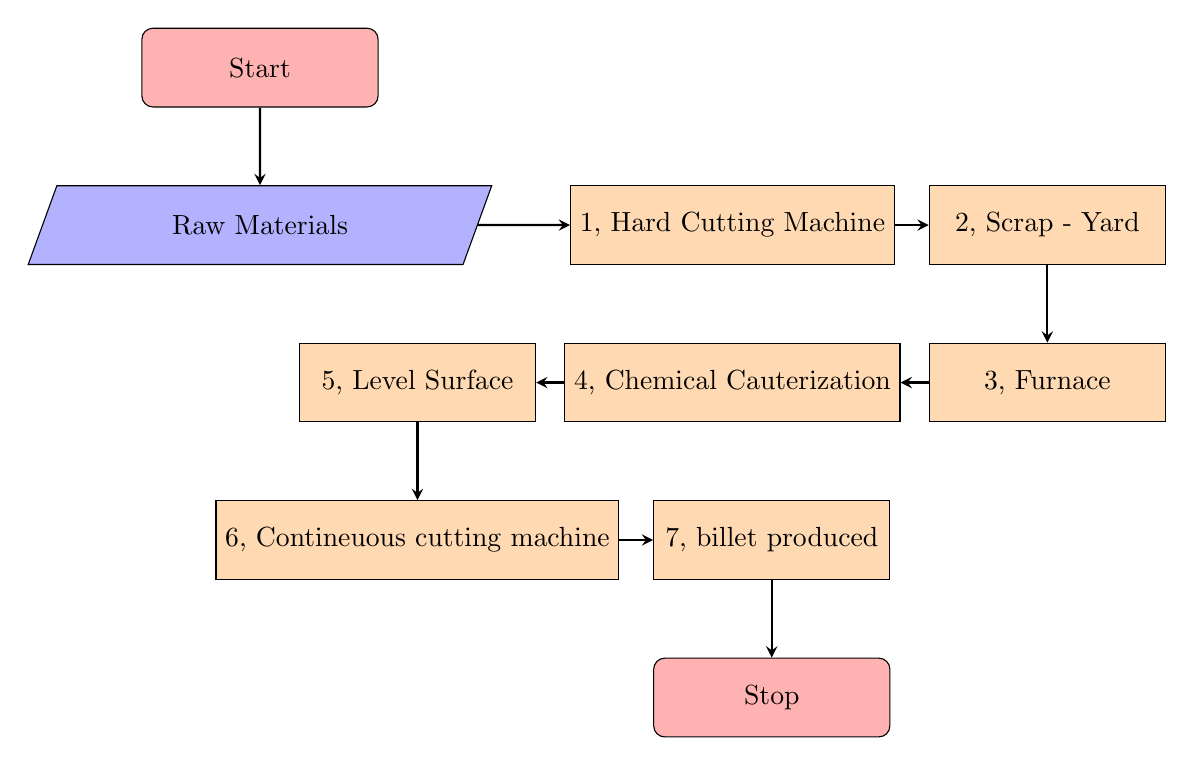
\begin{tikzpicture}[node distance = 2cm]
        	
        	\node[startstop,xshift = 2cm](start){Start};
        	\node[io,below of =start](input){Raw Materials};
        	\node[process,right of =input,xshift = 4cm](Process 1){1, Hard Cutting Machine};
        	\node[process,right of =Process 1,xshift = 2cm](Process 2){2, Scrap - Yard};
        	\node[process,below of =Process 2](Process 3){3, Furnace};
        	\node[process,left of =Process 3,xshift = -2 cm](Process 4){4, Chemical Cauterization};
        	\node[process,left of =Process 4,xshift = -2cm](Process 5){5, Level Surface};
        	\node[process,below of =Process 5](Process 6){6, Contineuous cutting machine};
        	\node[process,right of =Process 6,xshift = 2.5cm](Process 7){7, billet produced};
        	\node[startstop,below of =Process 7](stop){Stop};
        	
        	\draw [arrow](start)--(input);
			\draw [arrow](input)--(Process 1);
			\draw [arrow](Process 1)--(Process 2);
			\draw [arrow](Process 2)--(Process 3);
			\draw [arrow](Process 3)--(Process 4);
			\draw [arrow](Process 4)--(Process 5);
			\draw [arrow](Process 5)--(Process 6);
			\draw [arrow](Process 6)--(Process 7);
			\draw [arrow](Process 7)--(stop);
        	 
        	
        
        
        \end{tikzpicture}
        
             \begin{itemize}
        
\item(1){ 1 person control this step for proper cutting of raw materials}
\item(2){ after cutting 2 person takes the  materials from scrapyard to the furnace, the material is transferred to the furnace using a crane operated by one person } 
\item(3){ 2- 3 monitor and control the furnace }
\item(4){ 2 person apply chemical cauterization on the melted materials of the furnace}
\item(5){ 2 person level the melted materials coming from the furnace}
\item(6){ 2 person cuts the materials into equal chops of billet}
\item(7){ billet is produced}
\item{ transition between some of the process are done through crane which are operated by person}

        \end{itemize}
         \subsection{Drug international medicine}
        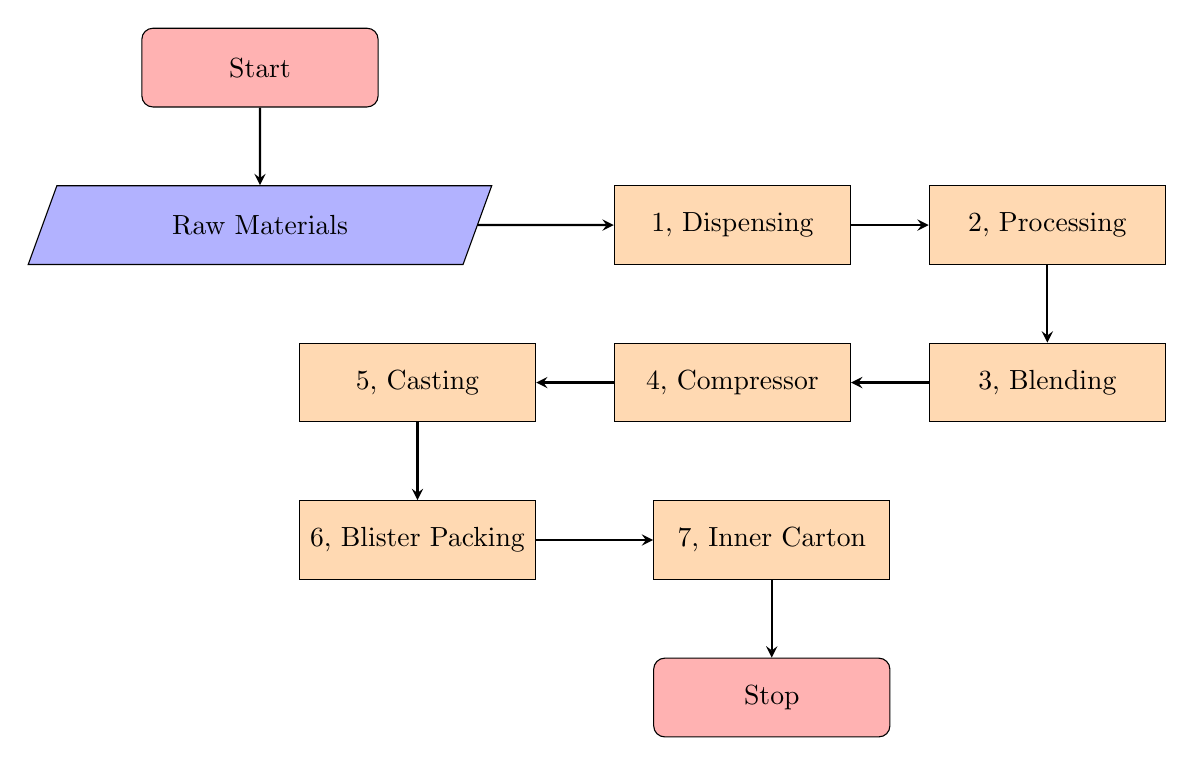
\begin{tikzpicture}[node distance = 2cm]
        	
        	\node[startstop,xshift = 2cm](start){Start};
        	\node[io,below of =start](input){Raw Materials};
        	\node[process,right of =input,xshift = 4cm](Process 1){1, Dispensing};
        	\node[process,right of =Process 1,xshift = 2cm](Process 2){2, Processing};
        	\node[process,below of =Process 2](Process 3){3, Blending};
        	\node[process,left of =Process 3,xshift = -2 cm](Process 4){4, Compressor};
        	\node[process,left of =Process 4,xshift = -2cm](Process 5){5, Casting};
        	\node[process,below of =Process 5](Process 6){6, Blister Packing};
        	\node[process,right of =Process 6,xshift = 2.5cm](Process 7){7, Inner Carton };
        	\node[startstop,below of =Process 7](stop){Stop};
        	
        	\draw [arrow](start)--(input);
			\draw [arrow](input)--(Process 1);
			\draw [arrow](Process 1)--(Process 2);
			\draw [arrow](Process 2)--(Process 3);
			\draw [arrow](Process 3)--(Process 4);
			\draw [arrow](Process 4)--(Process 5);
			\draw [arrow](Process 5)--(Process 6);
			\draw [arrow](Process 6)--(Process 7);
			\draw [arrow](Process 7)--(stop);
        	 
        	
        
        
        \end{tikzpicture}
        
             \begin{itemize}
        
\item(1){ 2 person control this step one weights the raw materials one takes the raw material to the next step }
\item(2){ 2 person maintains this step one drys the materials and the other puts in the blender} 
\item(3){ 1 person controls the blending }
\item(4){ 1 person controls the compression}
\item(5){ 3 person is assigned to casting}
\item(6){ 1 person operates the machine 2 person checks the blister packing}
\item(7){ 3 person checks the carton packing}


        \end{itemize}
        
\end{normalsize}
  
\end{document}